\documentclass[12pt]{article}
\usepackage{graphicx}
\usepackage{caption}
\usepackage{xcolor}
\usepackage{enumitem}
\usepackage{textgreek}

\linespread{1.25}

\title{Processing of Scalar Implicatures and Contextual and Lexical Cues} 

\author{}
\date{}

\begin{document} 
\maketitle 

\section{Methods}
\subsection*{Participants}
We recruited 2400 participants on Amazon Mechanical Turk (1200 per experiment). Participants were required to have a US IP address and a prior approval rating of $>$ 95\%. They were paid \$2.3.

\subsection*{Procedure and Materials}
Experiment 1 and Experiment 2 were identical except for the audio stimulus participants heard during the critical trials. In Experiment 2, the lack of partitive 'of' provided a lexical cue to the implicature. (CHANGE AFTER INTRO)

\paragraph{} At the beginning of each experiment, participants were assigned to one of the three groups and were presented with a different cover story. These cover stories were designed to establish an implicit QUD.

\paragraph{all QUD} Participants in all QUD group read a story explaining them that they are at a candy store and testing a row of special gumball machines. These gumball machines have 13 gumballs in their upper chambers and when they distribute gumballs, you see a certain number of gumballs move to the lower chamber. These machines also say how many gumballs you got (“You got X gumballs”), but are sometimes faulty in their report. The store worker’s boss has threatened to fire him if the gumball machines are left empty and he cannot see the machines from the register and only tell how full they are by their statements. Participants were asked to help the store worker by telling him if this statement is right or wrong by pressing the yes or no key. They were also told that they have 4 seconds to notify the store worker and they should make a decision as quickly as possible.

\begin{center}Is the machine empty? $\rightarrow$ Did I get all of the gumballs?\end{center}

\paragraph{any QUD} In the any QUD group, participants read the same story except, in their story, the store worker’s boss has threatened to fire him if the gumball machines get jammed. 

\begin{center}Is the machine jammed? $\rightarrow$ Did I get none of the gumballs?\end{center}

\paragraph{no QUD} Participants in the no QUD group didn’t read a cover story but instead read instructions that explained that they were going to see a gumball machine filled with gumballs and after a few seconds certain number of gumballs will move to its bottom chamber and the machine will say how many gumballs you got. Participants were asked to say if this statement right or wrong by pressing the yes or no key. They were told that they have 4 seconds to answer.

\begin{center}Is the statement correct? $\rightarrow$ No implicit QUD\end{center}

After reading the cover story, participants went through a scripted demonstration that showed various scenarios and the store worker’s reaction to their responses. In the all QUD condition, when all of gumballs dropped from the upper chamber to the lower chamber and the machine reported “You got all of the gumballs”, participants were asked to press the yes key and they read that they let the store worker know that the machine is empty and he therefore knows that he needs to refill the machine. They also read that one time someone got all of the gumballs and was told “You got all of the gumballs”, they pressed the no key and the store worker was fired because he didn’t refill the machine. In the any QUD condition, participants got no gumballs and the machine reported “You got none of the gumballs”. Participants were asked to press the yes key and read that they let the store worker know that the machine is not distributing gumballs and that he needs to fix the machine. They read that one time someone got 0 gumballs and was told “You got none of the gumballs”, they pressed the no key and the store worker was fired because he didn’t repair the machine. In the no QUD condition, the only feedback that participants got was a sentence that said whether they agreed or disagreed with the statement.

To ensure that participants paid attention to the cover story, participants in all QUD and any QUD conditions were asked a multiple-choice question about when the store worker will be fired. For the all QUD group the correct answer was “when the machines are empty” and for the any QUD group the correct answer was “when the machines jam. When participants answered this question incorrectly they were presented with the cover story again and went through the demonstration. Halfway through the experiment, participants were asked to answer this multiple-choice question again. This was done to prevent the decay of the implicit QUD over time. 

There were 4 practice trials with “You got all of the gumballs” and “You got none of the gumballs” statements. On 2 of these trials, the statement was correct, and on 2 of them it was incorrect. 

After the practice trials, there were 72 experimental trials. The number of gumballs in the lower chamber (0 to 13 gumballs) and the quantifier in the statement (some, none, all) were varied. On 32 of the trials the expected answer was yes, and on 32 of the trials the expected answer was no. \textbf{The remaining 8 trials were occurrences of the critical trial and the main focus of this experiment. On these trials, all thirteen of the gumballs dropped to the lower chamber. In experiment 1, participants heard the statement “You got some of the gumballs” and in Experiment 2, participants heard the statement "You got some gumballs".} (Note that in Experiment 2, on non-critical trials the simple 'some' was used). 

When participants agree with the statement "You got some (of the) gumballs", they interpret it semantically as "You got some, and possibly all of the gumballs" and when they disagree with the statement, they interpret it pragmatically as “You got some, but not all of the gumballs”. YES responses are considered semantic and NO responses are considered pragmatic responses.

% \begin{center}\textcolor{red}{INSERT TABLE HERE - STIMULI LIST}\end{center}

\pagebreak
\section{Results}

\subsection*{Exclusions}
Participants were excluded based on the criteria below. 

\begin{enumerate}[noitemsep]
\item non-native English speakers 
\item participants who get the second comprehension question wrong more than twice 
\item participants with accuracy of lower than 85\% on non-critical trials with quantifiers "some","none","all" and numbers below 6
\end{enumerate}

\begin{table}[h]
    \centering
    \caption {Number of participants excluded with each criterion}
    \begin{tabular}{ccccc}
    & Experiment 1 & Experiment 2 \\
    1 & 37 & 35 \\
    2 & 21 & 15 \\
    3 & 255 & 269 \\
    \textbf{total} & \textbf{313} & \textbf{321}* \\
    \end{tabular} 
\end{table}
\vspace{-6mm}
* one person participated twice, both attempts were removed.

\medskip

\begin{table}[h]
    \centering
    \caption {Number of participants in each group after exclusions}
    \begin{tabular}{ccccccc}
    & all QUD & any QUD & no QUD & \textbf{total}\\
    Experiment 1 & 288 & 280 & 319 & \textbf{887}\\
    Experiment 2 & 292 & 283 & 304 & \textbf{879}\\
    \end{tabular}
\end{table}

Additionally, trials with response times that are 2.5 standard deviations above the mean for that condition or that are faster than the onset of the quantifier were not included in the analysis. Only responses to critical trials are reported. 


\subsection*{Judgements}
Both the contextual support provided by the implicit QUD and the lexical cue (absence of partitive "of") affected the robustness of scalar implicatures. Absence of the partitive 'of' lead to more semantic responses regardless of the implicit QUD and relevance of the QUD lead to more pragmatic responses regardless of the presence of the lexical cue. In both experiments, participants in the all QUD group gave the most number of pragmatic responses and participants in the no QUD groups gave the least.

\begin{figure}[!ht]  
\begin{minipage}{.5\textwidth}
    \caption*{Experiment 1}
    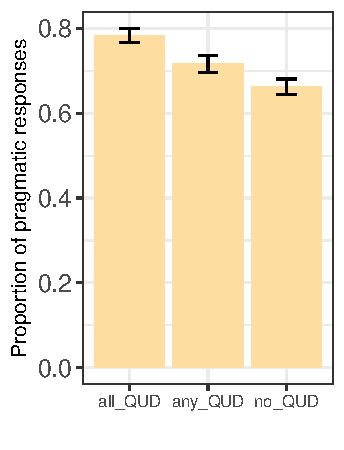
\includegraphics[height=7cm]{img/exp4_proportion_pragmatic.pdf}    
    \end{minipage}%
\begin{minipage}{.5\textwidth}
    \caption*{Experiment 2}
    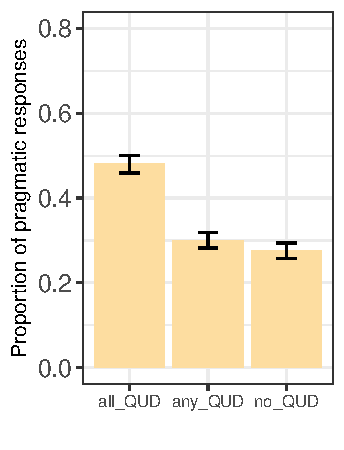
\includegraphics[height=7cm]{img/exp5_proportion_pragmatic.pdf}
    \end{minipage}%
    \caption{Proportion of pragmatic responses on critical trials}
\end{figure}

 A mixed effects logistic regression predicting response type with random by-participants intercepts from fixed effects of QUD found a main effect of QUD such that there are more pragmatic (NO) responses for all QUD compared to any QUD (Experiment 1: \textbeta=1.28, SE=0.52, p$>$0.0001, Experiment 2: \textbeta=3.81, SE=0.52, p$>$0.0001) and no QUD (Experiment 1: \textbeta=2.07, SE=0.63, p$>$0.0001, Experiment 2: \textbeta=3.45, SE=0.58, p$>$0.0001).

\begin{figure}[!ht] 
    \begin{minipage}{.5\textwidth}
    \caption*{Experiment 1}
    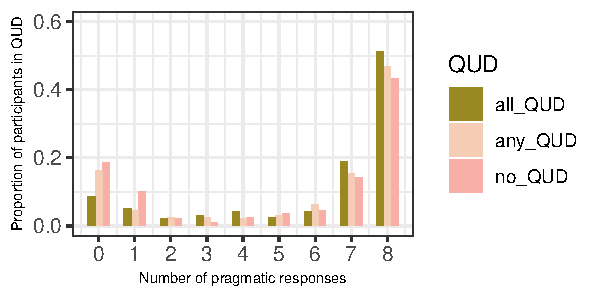
\includegraphics[height=4.6cm]{img/exp4_pragmatic_proportion.pdf}
    \end{minipage}%
    \begin{minipage}{.5\textwidth}
    \caption*{Experiment 2}
    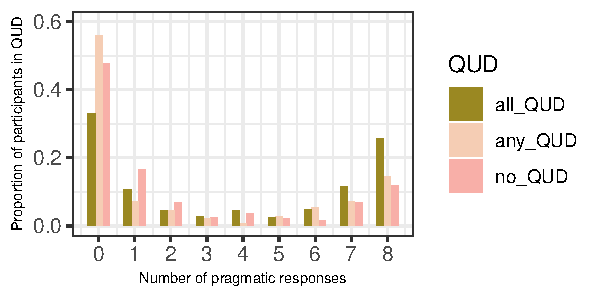
\includegraphics[height=4.6cm]{img/exp5_pragmatic_proportion.pdf}
    \end{minipage}%
    \caption{Distribution of participants over number of pragmatic responses on critical trials}
\end{figure}

\subsection*{Response Times}
Overall, the absence of the partitive lead to faster responses. When there was no implicit QUD and the partitive was present, pragmatic responses were faster than semantic ones, and when the simple some was used, semantic responses became faster than pragmatic ones. 

\begin{figure}[!ht] 
    \begin{minipage}{.5\textwidth}
        \caption*{Experiment 1}
        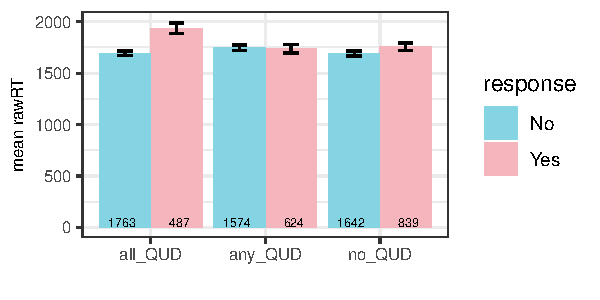
\includegraphics[height=4.3cm]{img/exp4_response_time.pdf}
    \end{minipage}%
    \begin{minipage}{.5\textwidth}
        \caption*{Experiment 2}
        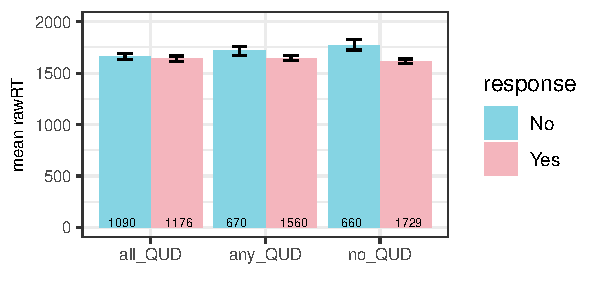
\includegraphics[height=4.3cm]{img/exp5_response_time.pdf}
    \end{minipage}%
    \caption{Mean response times for semantic and pragmatic responses on critical trials as a function of QUD}
\end{figure}

The QUD affected the response time for semantic and pragmatic responses differently. The more relevant the alternative, the faster the pragmatic responses became and the slower the semantic responses became. 

The two cues interacted in a way such that the absence of the partitive changed the faster response type in all QUD groups. The fastest responses were observed when 1) partitive was present, QUD was relevant and participants responded pragmatically and 2) partitive was absent, QUD was less relevant and participants responded semantically. 

A mixed effects linear regression model with random by-participant intercepts predicting log-transformed response time from fixed effects of QUD, response type and their interaction, revealed a main effect of response type such that NO responses were always faster than YES responses (\textbeta=1.28, SE=0.02, p$>$0.0001). The interaction between response type and QUD was also found to be significant such that in the all QUD group, NO responses were faster and YES responses were slower compared to any QUD group (\textbeta=-0.11, SE=0.02, p$>$0.0001) and no QUD group (\textbeta=-0.07, SE=0.02, p$>$0.001). Response type was centered before entering the analysis.

\subsection*{Responder Type}
In the post hoc analysis, participants were divided into two groups as semantic and pragmatic responders. We investigated whether responder type affect speed of processing differently for different responder groups and whether this is affected by contextual and lexical cues. Semantic responders are participants who gave semantic responses more than half of the time ($>$4) and pragmatic responders are participants who gave pragmatic responses more than half of the time. Participants who gave the same number of pragmatic and semantic responses were excluded from this visualization and analysis. 

\begin{figure}[!ht] 
    \begin{minipage}{.5\textwidth}
        \caption*{Experiment 1}
        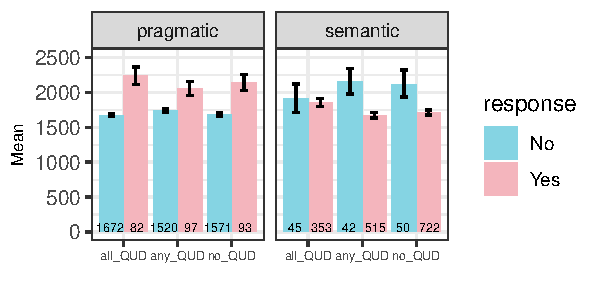
\includegraphics[height=4.4cm]{img/exp4_responder.pdf}
    \end{minipage}%
    \begin{minipage}{.5\textwidth}
        \caption*{Experiment 2}
        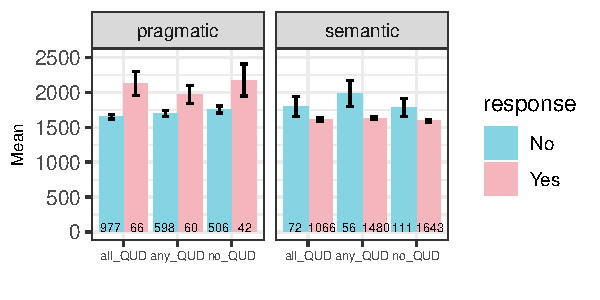
\includegraphics[height=4.4cm]{img/exp5_responder.pdf}
    \end{minipage}%
    \caption{Mean response times for semantic and pragmatic responders (inconsistent responders excluded)}
\end{figure}

In both experiments, and in each QUD group, pragmatic responders were faster to respond pragmatically and semantic responders were faster to respond semantically. The partitive didn't efect the response times of different responders signinficantly. However, with increasing relevance of the QUD, pragmatic responders got faster at responding pragmatically and semantic responders got slower in responding semantically.

We used a model selection to determine the best model that 

\begin{figure}[!ht] 
    \centering
    \caption*{Experiment 4}
    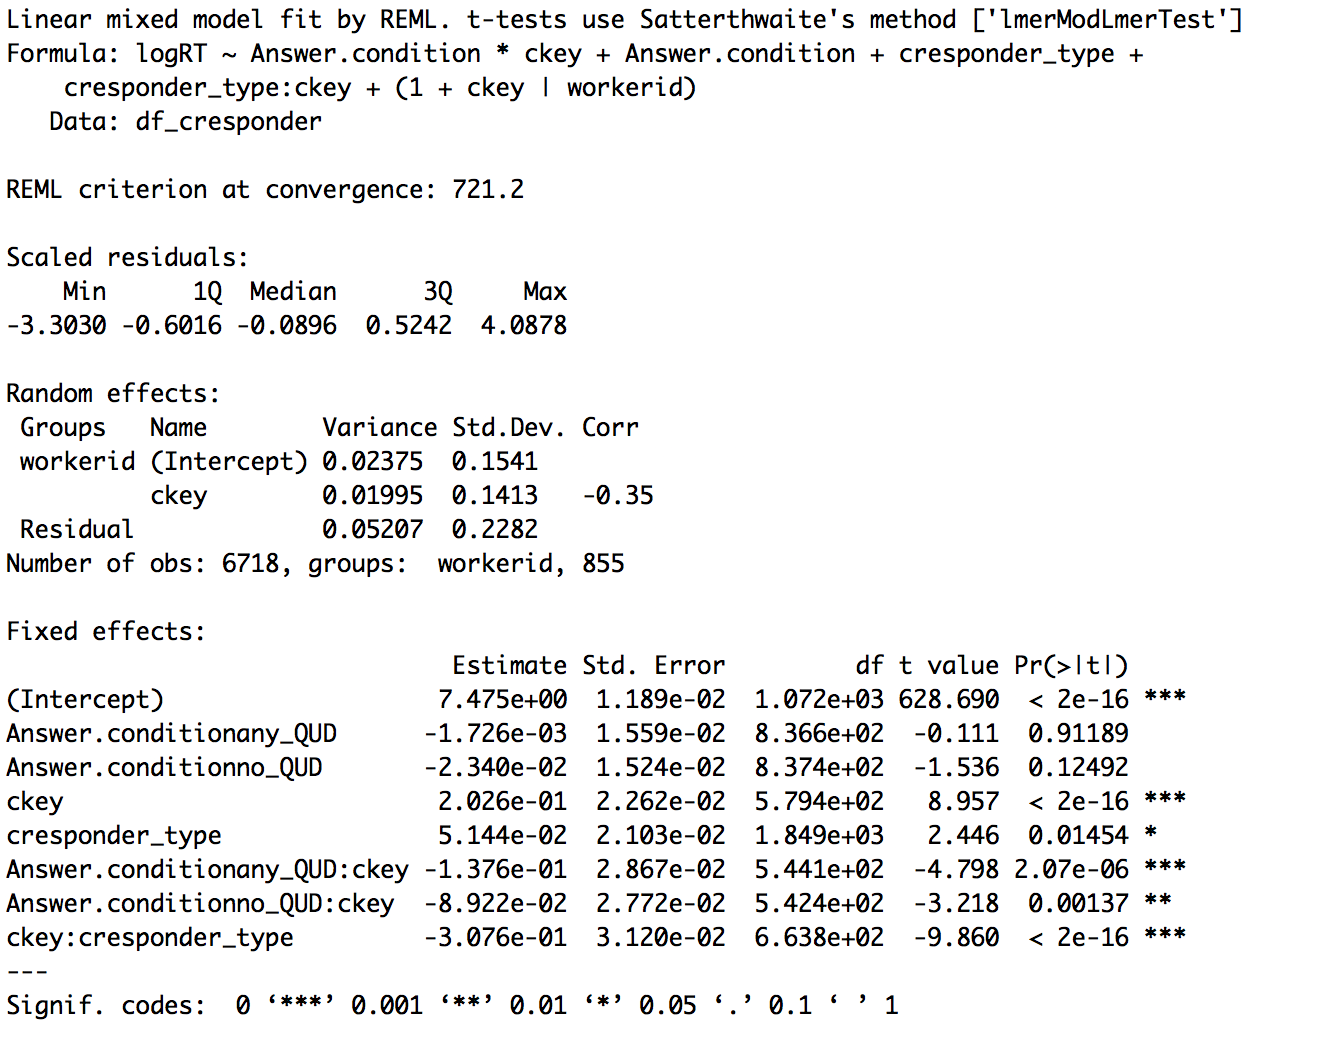
\includegraphics[height=12cm]{models/best_model}
\end{figure}

\pagebreak
% \section*{Formatting Citations}
\bibliography{scibib}
\bibliographystyle{Science}
\end{document}